%!TEX root = ../report.tex
\documentclass[report.tex]{subfiles}
\begin{document}
    \chapter{Solution}
    We discussed various kind of controllers in chapter \ref{State of the Art} session \ref{Controller} and the background knowledge of Popov-Vereshchagin hybrid solver in chapter \ref{Background}.In this chapter The proposed robot archtechture session will present how the forementioned sovler and controller implement on the robot. Session extension of Robif2b will discuss how to modify Robif2b such that the communication between robot and the software interface can be extended.

    \section{Proposed robot archtechture}

    Figure \ref{fig:sys} shows the robot system archtechture consist of a cascaded controller, the Popov-Vereshchagin solver and the robot. The cascaded controller consist of a P-position controller and a P-velocity controller. The main program fetch the instantaneous joint angle $q$ from the robot, then perform forward kinematic to compute the current Cartesian pose of the robot's end-effector $X_{curr}$. Then calculate the position error term $X_{err}$ by calling \textit{diff($X_{goal}$,$X_{curr}$)} mentioned in chapter \ref{diff_frame} where $X_{goal}$ is the desired pose of the robot's end-effector of the current task.
    \begin{figure}[h!]
        \centering
        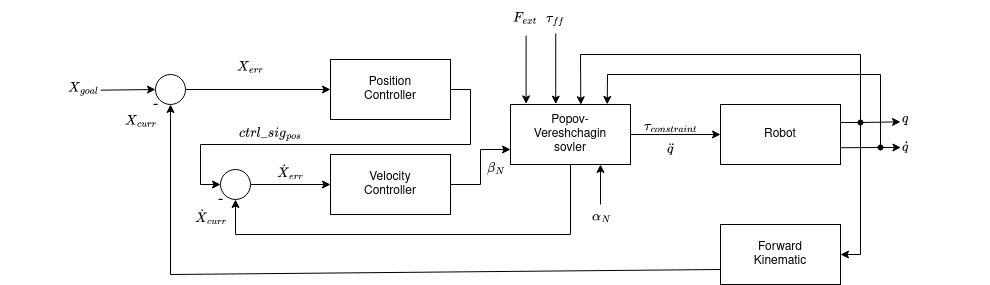
\includegraphics[width=1\linewidth]{images/systemdia.png}
        \caption{A generic control diagram illustrate the interactions of end-effector (task)
        pos and cascaded controllers with the constrained dynamics
        algorithm. It shows the connection between controller, solver and robot.}
        \label{fig:sys}
    \end{figure}
    \section{Extension of Robif2b}
\end{document}
